\documentclass[A4Page,11pt]{article}

%% Language and font encodings
\usepackage[english]{babel}
\usepackage[utf8x]{inputenc}
\usepackage[T1]{fontenc}
\usepackage{subcaption}
\usepackage{graphicx}

%% Sets page size and margins
\usepackage[a4paper,top=1.5cm,bottom=2cm,left=2cm,right=2cm,marginparwidth=1.75cm]
{geometry}

%% Useful packages
\usepackage{amsmath}
\usepackage{graphicx}
\usepackage[colorinlistoftodos]{todonotes}
\usepackage[colorlinks=true, allcolors=blue]{hyperref}


\title{\vspace{-2.0cm}Symbols, Patterns and Signals: CW1 Report}\vspace{-3ex}
\author{
    Aaron Wray\\
    \texttt{aw16997@my.bristol.ac.uk}
    \and
    Nick Broom\\
    \texttt{nb16568@my.bristol.ac.uk}
}

\begin{document}
\maketitle



\section{Introduction}

The aim of this assignment was to gain experience in the practices and methods involved in clustering and classifying data. There are many methods that can be used in achieving this goal; for clustering  some of these include connectivity, distribution, density and centroid based clustering. For classifying these include decision trees, neural networks, support vector machines, naïve Bayes and Bayesian belief networks. In our assignment, we looked to cluster our data using centroid based clustering and classify our data using two different approaches: a nearest centroid classifier and a maximum likelihood classifier. The nearest centroid classification generated three cluster centroids through use of the K Means algorithm on the training data. It then classified all the test data based on which centroid it was closest to. Using a maximum likelihood classifier was more complex as this required generating a multivariate normal distribution. Then we plotted the decision boundary as all the points in the plot which had an equal probability of belonging to two normal distributions. 

\section{Feature Selection}

Feature selection is a technique used in data classification, given a set of features/attributes, as input, we want a subset of features which allows us to classify the data in the best possible way. All extraneous attributes are then essentially discarded with in the model.\par

The training data that we were provided with contained 150 values for 5 different features in total. To begin with we plotted the data points of each feature against another. This resulted in a 5x5 matrix as seen below in Figure 1. It is important to note that leading diagonal of the matrix is a feature of the training data plotted against itself and that the graphs either side of the leading diagonal are equivalent, but with the axes switched. Upon visual inspection of the matrix below the graph in the 3rd column 2nd row or similarly, 2nd column 3rd row, hold the most significance. As they are the only combination of features that exhibit the training data grouped into 3 distinct clusters. Using this information, we selected theses features to generate our model.
\begin{figure}[h!]
\centering
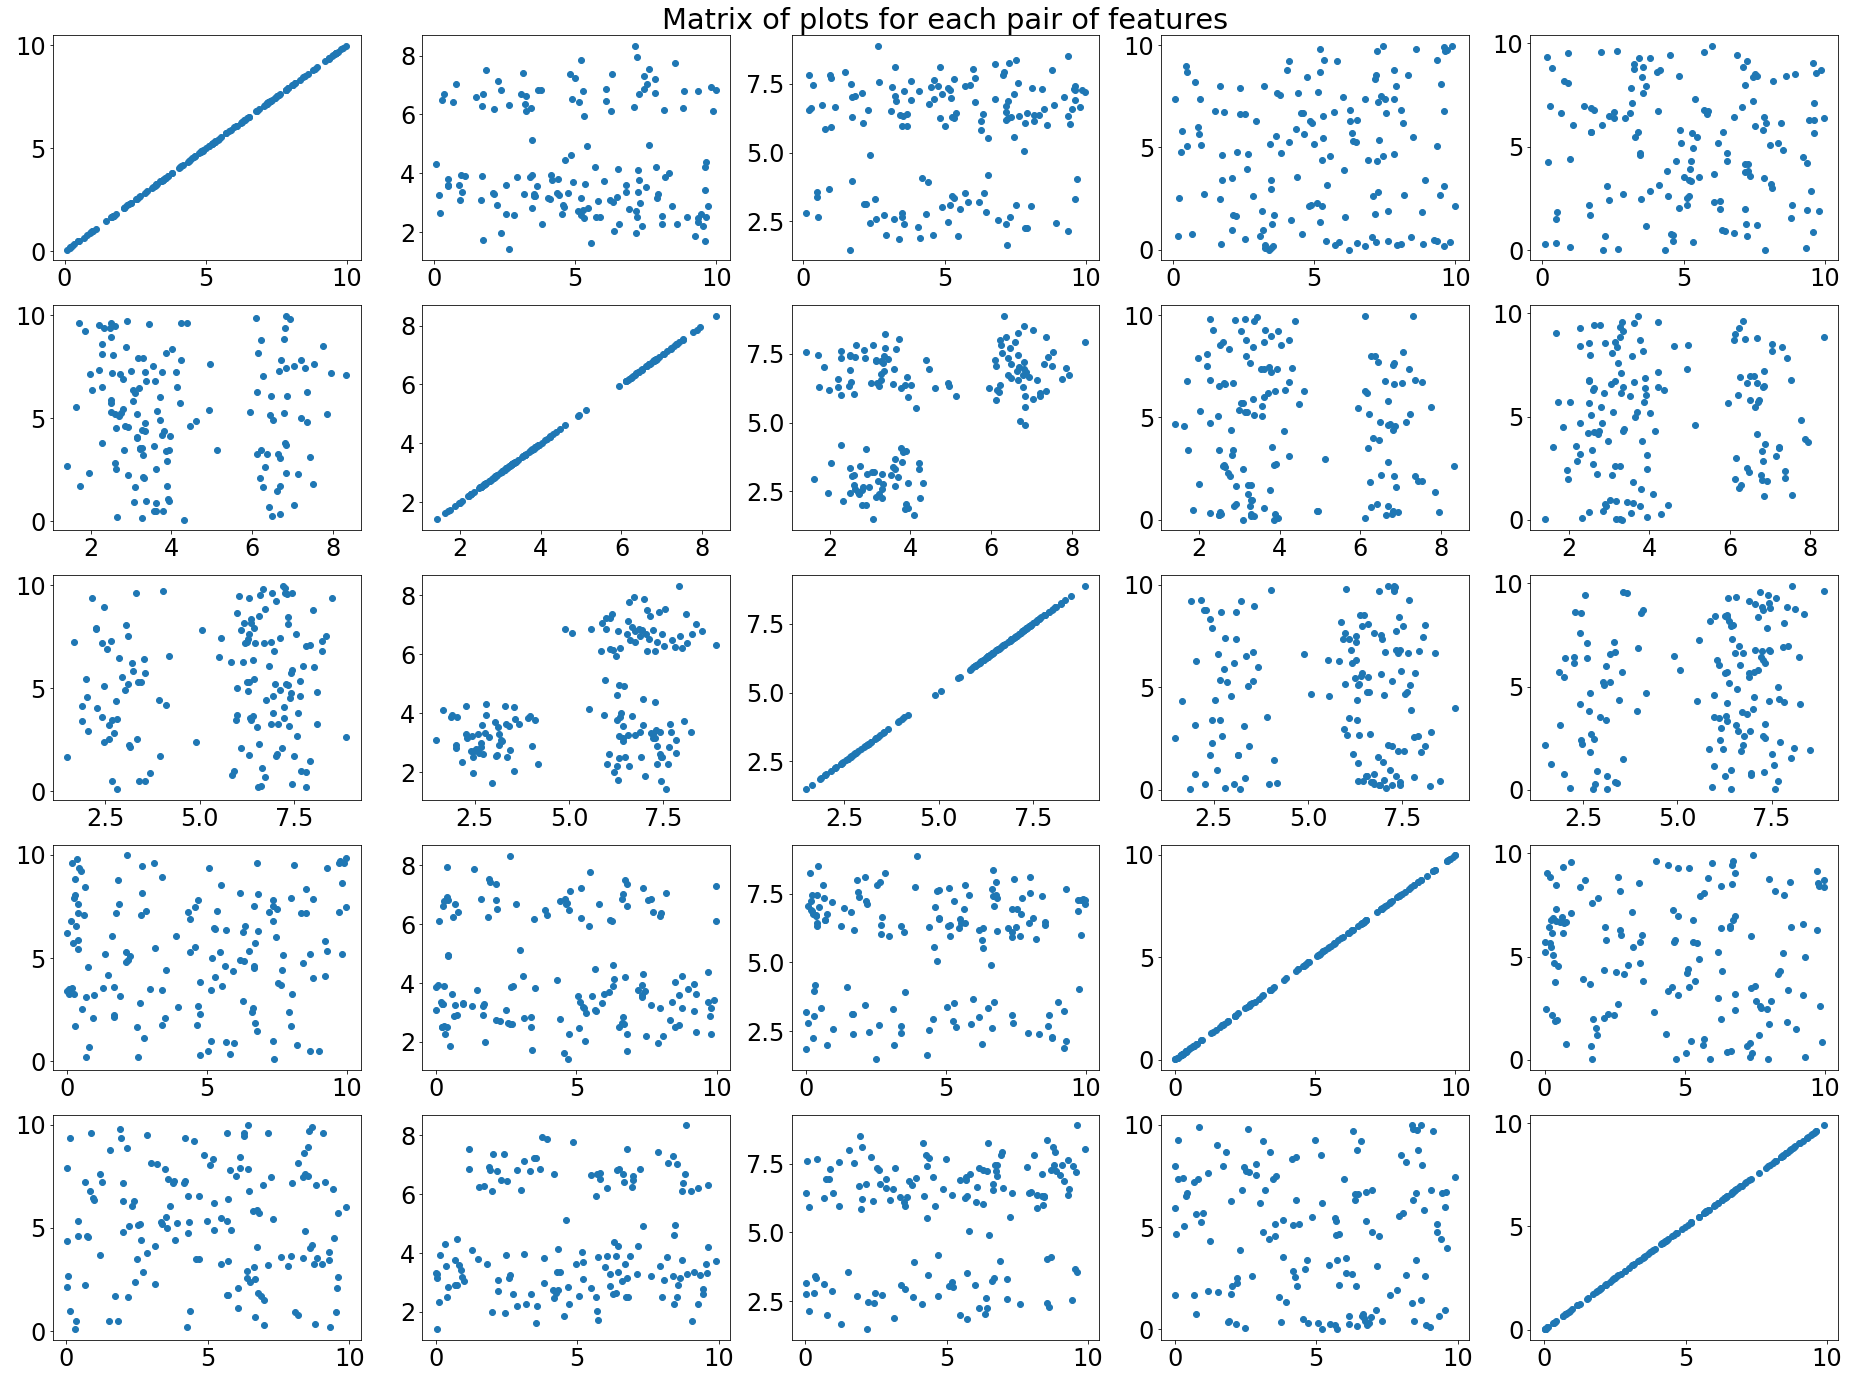
\includegraphics[width=0.65\linewidth]{download.png}
\caption{\label{fig 1:}Displays each feature of the training data plotted against each other}
\end{figure}



\section{Identifying the Classes}
As we plotted our selected features on a scatter diagram it became clear that there were 3 distinct clusters of data. To classify exactly which points belonged to each cluster we used the K-Means clustering algorithm. 
\begin{figure}[h!]
\centering
\includegraphics[width=0.65\linewidth]{fig_2.png}
\caption{\label{fig 2:}Displays our training data in three clusters and the centroid of each cluster}
\end{figure}

The K-Means algorithm returned to us three values. An array containing the centroids for each cluster, an array called labels that details which cluster each point belongs to and an inertia value which indicates how spread the data is within clusters. Next we had to use this labels array to create 3 new arrays containing all the points in each cluster. To do this we used the labels array in combination with the numpy.where() function to produce a list of indices for each cluster. We then made three copies of the training data and filtered each copy using the indices to get the points in each cluster.

\begin{figure}[h!]
\centering
\includegraphics[width=0.65\linewidth]{fig_3.png}
\caption{\label{fig 1:}Displays a non-optimal clustering of our training data by changing the initial configuration to the kmeans algorithm}
\end{figure}

We initially decided run the K-Means algorithm using the default parameters. After inspecting Figure 2 we were satisfied that the algorithm had correctly classified all the points. Therefore we didn’t feel the need to increase the iterations of the algorithm or the number of initial configurations for the cluster centres. \par

However, to show, the contrast of a non-optimal clustering we changed some of the initialization parameters of the K-Means algorithm to produce the result as shown in  \par

We manually inputted the initial cluster centres and deliberately made these non-optimal. We also ensured that this would be the only initial configuration of cluster centres the algorithm would use. Finally we reduced the number of iterations in the algorithm from 300 to 4 to ensure that the algorithm would not converge on an optimal solution. The non-optimality of the clustering in figure 3 can be seen by the fact that some clusters are much larger than others and that in two of the clusters they are large gaps in the middle of the cluster with no data points. \par

Further evidence that this is non-optimal clusters comes when we compare the inertia values of the two clusters. Where the total inertia represents the sum of all the distances between a data point and its cluster centre squared. The inertial value of the optimal clustering is 150.18 compared with 513.13 in the non-optimal clustering.


\section{Nearest Centroid Classification}
Once we had put our training data into three distinct clusters through use of the K means function we then had to classify all our test data based upon which centroid was the closest. To do this we used the cdist function to find the euclidean distance between each data point and the three centroids. Following this we used the numpy.argmin() function to return a 0, 1 or 2 for each data point based on whether it was closest to cluster 1,2 or 3.\par 

We realised that the information we had and the result we were looking for was similar to the problem of identifying the classes given a set of labels. So we went back in our program and generalised part of our question 2 by making a function that given a set of labels and some data points would put the data points into clusters. Then a further function to plot these clusters on our figure to avoid repeating similar code.\par

After we plotted the test data points on the graph we then plotted the decision boundary which is shown by the dotted lines in figure 4. All the points on the dotted lines represent all the points on the plot which are equidistant from two cluster centres. With the orange dot at the intersection of the three dotted lines representing the point which is equidistant from all three decision boundaries. 
\begin{figure}[h!]
\centering
\includegraphics[width=0.65\linewidth]{fig_4.png}
\caption{\label{fig 4:}Displays our training and test data with a nearest centroid classifier}
\end{figure}
We initially used the euclidean distance as our distance measure but after researching the documentation for cdist we found that there are 21 other methods for calculating the distance between between two vectors. So we decided to test two other distance measures, the Canberra and Manhattan distances. The equation below will calculate the Canberra distance between two vectors p and q:

\[d(p,q) = \sum_{i=1}^{n} \frac{|p_i - q_i|}{|p_i| + |q_i|}\]

Whereas the following equation will compute the cityblock or manhattan distance between two vectors p and q.

\[d(p,q) = \sum_{i=1}^{n} {|p_i - q_i|}\]
 
% \subsection{How to write Mathematics}

% \LaTeX{} is great at typesetting mathematics. Let $X_1, X_2, \ldots, X_n$ be a sequence of independent and identically distributed random variables with $\text{E}[X_i] = \mu$ and $\text{Var}[X_i] = \sigma^2 < \infty$, and let
% \[S_n = \frac{X_1 + X_2 + \cdots + X_n}{n}
%       = \frac{1}{n}\sum_{i}^{n} X_i\]
% denote their mean. Then as $n$ approaches infinity, the random variables $\sqrt{n}(S_n - \mu)$ converge in distribution to a normal $\mathcal{N}(0, \sigma^2)$.

However as is evident in the diagram most of our test data points lie quite far from the nearest centroid decision boundary and so therefore changing between these different distance measures didn’t change any classifications.

\section{Maximum Likelihood Classifier}
In order to produce a maximum likelihood classifier for our clusters we need to model each cluster using a two dimensional normal distribution. We started by calculating the mean, a row vector of length 2 and the covariance, which was a 2x2 matrix. The next step for each cluster was to generate a large series of evenly spaced samples between 1 and 10 in the x axis and y axis. Then we calculated the probability that each sample belonged to a particular normal distribution, using the probability density function that required the mean, covariance and a single sample as an input. The result of this was a 2x2 matrix that contained the probabilities that each sample existed within the two dimensional normal distribution of a particular cluster, we labelled this as the ‘z’ values for that cluster.
The equation for the two dimensional normal distribution is written as:

%  $\text{E}[X_i] = \mu$ and $\text{Var}[X_i] = \sigma^2 < \infty$, and let
% \[S_n = \frac{X_1 + X_2 + \cdots + X_n}{n}
%       = \frac{1}{2\pi}\sum_{i}^{n} X_i\]
\[f(x)   = \frac{exp( -\frac{1}{2} (x - \mu)^ T \Sigma ^{-1} (x - \mu))}{2\pi |\Sigma|}\]
     
% $\mathcal{N}(0, \sigma^2)$.

In this equation x is a 2 component column vector, which represents all the combinations of our evenly spaced samples for x and y that were generated earlier in the question. \(\mu\) is mean and  \(\Sigma\) is the covariance, as described before. |\(\Sigma\)| and \(\Sigma ^{-1}\) are its determinant and inverse.(Reference this). The part of the equation that is raised to the exponent, \(-\frac{1}{2} (x - \mu)^ T \Sigma ^{-1} (x - \mu)\) is the formula used to calculate the mahalanobis distance. The mahalonbis distance, in this case is the distance between the centroid and a data point and is used later on to identify outliers in our data.

\begin{figure}[h!]
\centering
\includegraphics[width=0.65\linewidth]{fig_5.png}
\caption{\label{fig 5:}displays the maximum likelihood boundaries between clusters along with the nearest centroid boundaries
}
\end{figure}

We then obtained the maximum likelihood decision boundary between each cluster by subtracting the ‘z’ values. This can been seen visibly in fig 5.1, as the difference was plotted as a contour, giving a non linear decision boundary between each cluster. The hyperbolic decision boundaries that  indicates that each cluster have different covariances. In order to have our maximum likelihood decision boundary match our nearest centroid decision boundary all we had to do was set the covariance to be the identity matrix rather than generating it from the cluster data. \par

To compare between the non-linear and linear decision boundaries we plotted them on the same graph. When examining the data, it appears that the non-linear and linear decision boundaries disagree. Two points in cluster 2 of the training data lie on the cluster 3 side of the non-linear decision boundary. \par

In this instance there seems to be a compromise between the complexity and tractability of the two different classification methods used. The simpler nearest centroid classification seems to perform better than the more complex maximum likelihood classification,as it over fits the model to the data.

\section{Discussion of Results}
On the final part of our assignment we produced a MAP estimation given a set of prior probabilities. By making one cluster twice as likely as another the impact on the decision boundaries wasn’t too significant so we also decided to investigate the impact of making one cluster 10 times as likely as the other clusters with the results shown below in figure 6.

\begin{figure}[h!]
  \centering
  \begin{subfigure}[b]{0.45\linewidth}
    \includegraphics[width=\linewidth]{fig_6.png}
     \caption{Cluster 2 is twice as likely.}
  \end{subfigure}
  \begin{subfigure}[b]{0.45\linewidth}
    \includegraphics[width=\linewidth]{fig_7.png}
    \caption{Cluster 2 is ten times as likely.}
  \end{subfigure}
  \caption{MAP classifier based on prior probabilities .}
  \label{fig:coffee3}
\end{figure}

As is evident in the diagram when we give cluster 1 a prior probability of twice the other cluster the shift in the decision boundary isn’t too significant. However, when we make cluster 1 ten times more likely than the other clusters there is a significant shift in the decision boundary and one piece of training data that was previously in cluster 1 will now be in cluster 3.

\begin{figure}[h!]
\centering
\includegraphics[width=0.65\linewidth]{fig_10.png}
\caption{\label{fig 1:}}
\end{figure}

When we modelled our clusters on a normal distribution wanted to see how many of our points were included within 95\% of the probability mass for each cluster. Using the Chi squared distribution you can derive that this is equivalent to drawing an ellipsis with Mahalanobis distance of 6. By drawing these ellipsis we can see that cluster 3 has significantly more outliers in the data as there are 3 data points lying outside the 95\% line compared with 0 for Cluster 2.  A future improvement of the maximum likelihood classification model could be to first check which training points lie outside of the 95\% probability mass and remove them from the training data. 


% \subsection{How to add Citations and a References List}

% You can upload a \verb|.bib| file containing your BibTeX entries, created with JabRef; or import your \href{https://www.overleaf.com/blog/184}{Mendeley}, CiteULike or Zotero library as a \verb|.bib| file. You can then cite entries from it, like this: \cite{greenwade93}. Just remember to specify a bibliography style, as well as the filename of the \verb|.bib|.

% You can find a \href{https://www.overleaf.com/help/97-how-to-include-a-bibliography-using-bibtex}{video tutorial here} to learn more about BibTeX.

% We hope you find Overleaf useful, and please let us know if you have any feedback using the help menu above --- or use the contact form at \url{https://www.overleaf.com/contact}!

% \bibliographystyle{alpha}
% \bibliography{sample}

\end{document}